% Options for packages loaded elsewhere
\PassOptionsToPackage{unicode}{hyperref}
\PassOptionsToPackage{hyphens}{url}
\PassOptionsToPackage{dvipsnames,svgnames,x11names}{xcolor}
%
\documentclass[
  letterpaper,
  DIV=11,
  numbers=noendperiod]{scrreprt}

\usepackage{amsmath,amssymb}
\usepackage{lmodern}
\usepackage{iftex}
\ifPDFTeX
  \usepackage[T1]{fontenc}
  \usepackage[utf8]{inputenc}
  \usepackage{textcomp} % provide euro and other symbols
\else % if luatex or xetex
  \usepackage{unicode-math}
  \defaultfontfeatures{Scale=MatchLowercase}
  \defaultfontfeatures[\rmfamily]{Ligatures=TeX,Scale=1}
\fi
% Use upquote if available, for straight quotes in verbatim environments
\IfFileExists{upquote.sty}{\usepackage{upquote}}{}
\IfFileExists{microtype.sty}{% use microtype if available
  \usepackage[]{microtype}
  \UseMicrotypeSet[protrusion]{basicmath} % disable protrusion for tt fonts
}{}
\makeatletter
\@ifundefined{KOMAClassName}{% if non-KOMA class
  \IfFileExists{parskip.sty}{%
    \usepackage{parskip}
  }{% else
    \setlength{\parindent}{0pt}
    \setlength{\parskip}{6pt plus 2pt minus 1pt}}
}{% if KOMA class
  \KOMAoptions{parskip=half}}
\makeatother
\usepackage{xcolor}
\setlength{\emergencystretch}{3em} % prevent overfull lines
\setcounter{secnumdepth}{5}
% Make \paragraph and \subparagraph free-standing
\ifx\paragraph\undefined\else
  \let\oldparagraph\paragraph
  \renewcommand{\paragraph}[1]{\oldparagraph{#1}\mbox{}}
\fi
\ifx\subparagraph\undefined\else
  \let\oldsubparagraph\subparagraph
  \renewcommand{\subparagraph}[1]{\oldsubparagraph{#1}\mbox{}}
\fi

\usepackage{color}
\usepackage{fancyvrb}
\newcommand{\VerbBar}{|}
\newcommand{\VERB}{\Verb[commandchars=\\\{\}]}
\DefineVerbatimEnvironment{Highlighting}{Verbatim}{commandchars=\\\{\}}
% Add ',fontsize=\small' for more characters per line
\usepackage{framed}
\definecolor{shadecolor}{RGB}{241,243,245}
\newenvironment{Shaded}{\begin{snugshade}}{\end{snugshade}}
\newcommand{\AlertTok}[1]{\textcolor[rgb]{0.68,0.00,0.00}{#1}}
\newcommand{\AnnotationTok}[1]{\textcolor[rgb]{0.37,0.37,0.37}{#1}}
\newcommand{\AttributeTok}[1]{\textcolor[rgb]{0.40,0.45,0.13}{#1}}
\newcommand{\BaseNTok}[1]{\textcolor[rgb]{0.68,0.00,0.00}{#1}}
\newcommand{\BuiltInTok}[1]{\textcolor[rgb]{0.00,0.23,0.31}{#1}}
\newcommand{\CharTok}[1]{\textcolor[rgb]{0.13,0.47,0.30}{#1}}
\newcommand{\CommentTok}[1]{\textcolor[rgb]{0.37,0.37,0.37}{#1}}
\newcommand{\CommentVarTok}[1]{\textcolor[rgb]{0.37,0.37,0.37}{\textit{#1}}}
\newcommand{\ConstantTok}[1]{\textcolor[rgb]{0.56,0.35,0.01}{#1}}
\newcommand{\ControlFlowTok}[1]{\textcolor[rgb]{0.00,0.23,0.31}{#1}}
\newcommand{\DataTypeTok}[1]{\textcolor[rgb]{0.68,0.00,0.00}{#1}}
\newcommand{\DecValTok}[1]{\textcolor[rgb]{0.68,0.00,0.00}{#1}}
\newcommand{\DocumentationTok}[1]{\textcolor[rgb]{0.37,0.37,0.37}{\textit{#1}}}
\newcommand{\ErrorTok}[1]{\textcolor[rgb]{0.68,0.00,0.00}{#1}}
\newcommand{\ExtensionTok}[1]{\textcolor[rgb]{0.00,0.23,0.31}{#1}}
\newcommand{\FloatTok}[1]{\textcolor[rgb]{0.68,0.00,0.00}{#1}}
\newcommand{\FunctionTok}[1]{\textcolor[rgb]{0.28,0.35,0.67}{#1}}
\newcommand{\ImportTok}[1]{\textcolor[rgb]{0.00,0.46,0.62}{#1}}
\newcommand{\InformationTok}[1]{\textcolor[rgb]{0.37,0.37,0.37}{#1}}
\newcommand{\KeywordTok}[1]{\textcolor[rgb]{0.00,0.23,0.31}{#1}}
\newcommand{\NormalTok}[1]{\textcolor[rgb]{0.00,0.23,0.31}{#1}}
\newcommand{\OperatorTok}[1]{\textcolor[rgb]{0.37,0.37,0.37}{#1}}
\newcommand{\OtherTok}[1]{\textcolor[rgb]{0.00,0.23,0.31}{#1}}
\newcommand{\PreprocessorTok}[1]{\textcolor[rgb]{0.68,0.00,0.00}{#1}}
\newcommand{\RegionMarkerTok}[1]{\textcolor[rgb]{0.00,0.23,0.31}{#1}}
\newcommand{\SpecialCharTok}[1]{\textcolor[rgb]{0.37,0.37,0.37}{#1}}
\newcommand{\SpecialStringTok}[1]{\textcolor[rgb]{0.13,0.47,0.30}{#1}}
\newcommand{\StringTok}[1]{\textcolor[rgb]{0.13,0.47,0.30}{#1}}
\newcommand{\VariableTok}[1]{\textcolor[rgb]{0.07,0.07,0.07}{#1}}
\newcommand{\VerbatimStringTok}[1]{\textcolor[rgb]{0.13,0.47,0.30}{#1}}
\newcommand{\WarningTok}[1]{\textcolor[rgb]{0.37,0.37,0.37}{\textit{#1}}}

\providecommand{\tightlist}{%
  \setlength{\itemsep}{0pt}\setlength{\parskip}{0pt}}\usepackage{longtable,booktabs,array}
\usepackage{calc} % for calculating minipage widths
% Correct order of tables after \paragraph or \subparagraph
\usepackage{etoolbox}
\makeatletter
\patchcmd\longtable{\par}{\if@noskipsec\mbox{}\fi\par}{}{}
\makeatother
% Allow footnotes in longtable head/foot
\IfFileExists{footnotehyper.sty}{\usepackage{footnotehyper}}{\usepackage{footnote}}
\makesavenoteenv{longtable}
\usepackage{graphicx}
\makeatletter
\def\maxwidth{\ifdim\Gin@nat@width>\linewidth\linewidth\else\Gin@nat@width\fi}
\def\maxheight{\ifdim\Gin@nat@height>\textheight\textheight\else\Gin@nat@height\fi}
\makeatother
% Scale images if necessary, so that they will not overflow the page
% margins by default, and it is still possible to overwrite the defaults
% using explicit options in \includegraphics[width, height, ...]{}
\setkeys{Gin}{width=\maxwidth,height=\maxheight,keepaspectratio}
% Set default figure placement to htbp
\makeatletter
\def\fps@figure{htbp}
\makeatother
\newlength{\cslhangindent}
\setlength{\cslhangindent}{1.5em}
\newlength{\csllabelwidth}
\setlength{\csllabelwidth}{3em}
\newlength{\cslentryspacingunit} % times entry-spacing
\setlength{\cslentryspacingunit}{\parskip}
\newenvironment{CSLReferences}[2] % #1 hanging-ident, #2 entry spacing
 {% don't indent paragraphs
  \setlength{\parindent}{0pt}
  % turn on hanging indent if param 1 is 1
  \ifodd #1
  \let\oldpar\par
  \def\par{\hangindent=\cslhangindent\oldpar}
  \fi
  % set entry spacing
  \setlength{\parskip}{#2\cslentryspacingunit}
 }%
 {}
\usepackage{calc}
\newcommand{\CSLBlock}[1]{#1\hfill\break}
\newcommand{\CSLLeftMargin}[1]{\parbox[t]{\csllabelwidth}{#1}}
\newcommand{\CSLRightInline}[1]{\parbox[t]{\linewidth - \csllabelwidth}{#1}\break}
\newcommand{\CSLIndent}[1]{\hspace{\cslhangindent}#1}

\KOMAoption{captions}{tableheading}
\makeatletter
\@ifpackageloaded{tcolorbox}{}{\usepackage[many]{tcolorbox}}
\@ifpackageloaded{fontawesome5}{}{\usepackage{fontawesome5}}
\definecolor{quarto-callout-color}{HTML}{909090}
\definecolor{quarto-callout-note-color}{HTML}{0758E5}
\definecolor{quarto-callout-important-color}{HTML}{CC1914}
\definecolor{quarto-callout-warning-color}{HTML}{EB9113}
\definecolor{quarto-callout-tip-color}{HTML}{00A047}
\definecolor{quarto-callout-caution-color}{HTML}{FC5300}
\definecolor{quarto-callout-color-frame}{HTML}{acacac}
\definecolor{quarto-callout-note-color-frame}{HTML}{4582ec}
\definecolor{quarto-callout-important-color-frame}{HTML}{d9534f}
\definecolor{quarto-callout-warning-color-frame}{HTML}{f0ad4e}
\definecolor{quarto-callout-tip-color-frame}{HTML}{02b875}
\definecolor{quarto-callout-caution-color-frame}{HTML}{fd7e14}
\makeatother
\makeatletter
\makeatother
\makeatletter
\@ifpackageloaded{bookmark}{}{\usepackage{bookmark}}
\makeatother
\makeatletter
\@ifpackageloaded{caption}{}{\usepackage{caption}}
\AtBeginDocument{%
\ifdefined\contentsname
  \renewcommand*\contentsname{Table of contents}
\else
  \newcommand\contentsname{Table of contents}
\fi
\ifdefined\listfigurename
  \renewcommand*\listfigurename{List of Figures}
\else
  \newcommand\listfigurename{List of Figures}
\fi
\ifdefined\listtablename
  \renewcommand*\listtablename{List of Tables}
\else
  \newcommand\listtablename{List of Tables}
\fi
\ifdefined\figurename
  \renewcommand*\figurename{Figure}
\else
  \newcommand\figurename{Figure}
\fi
\ifdefined\tablename
  \renewcommand*\tablename{Table}
\else
  \newcommand\tablename{Table}
\fi
}
\@ifpackageloaded{float}{}{\usepackage{float}}
\floatstyle{ruled}
\@ifundefined{c@chapter}{\newfloat{codelisting}{h}{lop}}{\newfloat{codelisting}{h}{lop}[chapter]}
\floatname{codelisting}{Listing}
\newcommand*\listoflistings{\listof{codelisting}{List of Listings}}
\makeatother
\makeatletter
\@ifpackageloaded{caption}{}{\usepackage{caption}}
\@ifpackageloaded{subcaption}{}{\usepackage{subcaption}}
\makeatother
\makeatletter
\@ifpackageloaded{tcolorbox}{}{\usepackage[many]{tcolorbox}}
\makeatother
\makeatletter
\@ifundefined{shadecolor}{\definecolor{shadecolor}{rgb}{.97, .97, .97}}
\makeatother
\makeatletter
\makeatother
\ifLuaTeX
  \usepackage{selnolig}  % disable illegal ligatures
\fi
\IfFileExists{bookmark.sty}{\usepackage{bookmark}}{\usepackage{hyperref}}
\IfFileExists{xurl.sty}{\usepackage{xurl}}{} % add URL line breaks if available
\urlstyle{same} % disable monospaced font for URLs
\hypersetup{
  pdftitle={Fundamental Epidemiological Study Designs},
  pdfauthor={Manh Nguyen Duc},
  colorlinks=true,
  linkcolor={blue},
  filecolor={Maroon},
  citecolor={Blue},
  urlcolor={Blue},
  pdfcreator={LaTeX via pandoc}}

\title{Fundamental Epidemiological Study Designs}
\author{Manh Nguyen Duc}
\date{3/20/25}

\begin{document}
\maketitle
\ifdefined\Shaded\renewenvironment{Shaded}{\begin{tcolorbox}[boxrule=0pt, enhanced, breakable, borderline west={3pt}{0pt}{shadecolor}, interior hidden, sharp corners, frame hidden]}{\end{tcolorbox}}\fi

\renewcommand*\contentsname{Table of contents}
{
\hypersetup{linkcolor=}
\setcounter{tocdepth}{2}
\tableofcontents
}
\bookmarksetup{startatroot}

\hypertarget{preface}{%
\chapter*{Preface}\label{preface}}
\addcontentsline{toc}{chapter}{Preface}

\markboth{Preface}{Preface}

I am on a journey to pursue my master's degree. I started writing this
notes as a way to summarize what I have learned from the course. It will
be basic and may contain some errors or mistakes. If you have time to go
through it, I would be grateful for your feedback. Most of the content
here is taken from the Distant Learning Epidemiology Master's Programme
provided by
\href{https://www.lshtm.ac.uk/study/courses/masters-degrees/epidemiology-online\#overview}{London
School of Hygene and Tropical Medicine} (LSHTM), with some modifications
taken from the book Modern Epidemiology, 4th edition (Lash et al. 2021)
and the Introduction to Biostatistics course provided by Prof.~Ronald
Geskus and his team at Oxford University Clinical Research Unit, Ho Chi
Minh.

Special thanks to \href{https://drthinhong.com/}{Dr.~Thinh Ong} for
motivating me to work on this.

\bookmarksetup{startatroot}

\hypertarget{introduction}{%
\chapter*{Introduction}\label{introduction}}
\addcontentsline{toc}{chapter}{Introduction}

\markboth{Introduction}{Introduction}

\textbf{Epidemiology} is a young science that has developed particularly
rapidly over the last 50 years, as new techniques of analysis have been
developed. Much progress has been made, particularly in understanding
the causes of ``non-communicable'' diseases (for example, the links
between H.pylori and gastric ulcer, and between EBV (Epstein-Barr virus)
and Burkitts lymphoma).

However new challenges continue to emerge. In recent decades, severe
acute respiratory syndrome (SARS), drug resistant tuberculosis and
methicillin-resistant \emph{staphylococcus aureus} (MRSA) have all
emerged as challenges to the public health. As an epidemiologist, you
are unlikely to become bored!

Source:
\href{https://www.lshtm.ac.uk/study/courses/masters-degrees/epidemiology-online\#overview}{EPM
101 LSHTM}

\part{Basic concepts}

\hypertarget{fundamental-epidemiology}{%
\chapter{Fundamental epidemiology}\label{fundamental-epidemiology}}

\begin{quote}
``The study of the occurrence and distribution of health-related events,
states, and processes in specified populations, including the study of
the determinants influencing such processes, and the application of this
knowledge to control relevant health problems.'' (Porta 2014)
\end{quote}

\begin{figure}

\begin{minipage}[b]{0.50\linewidth}

{\centering 

\raisebox{-\height}{

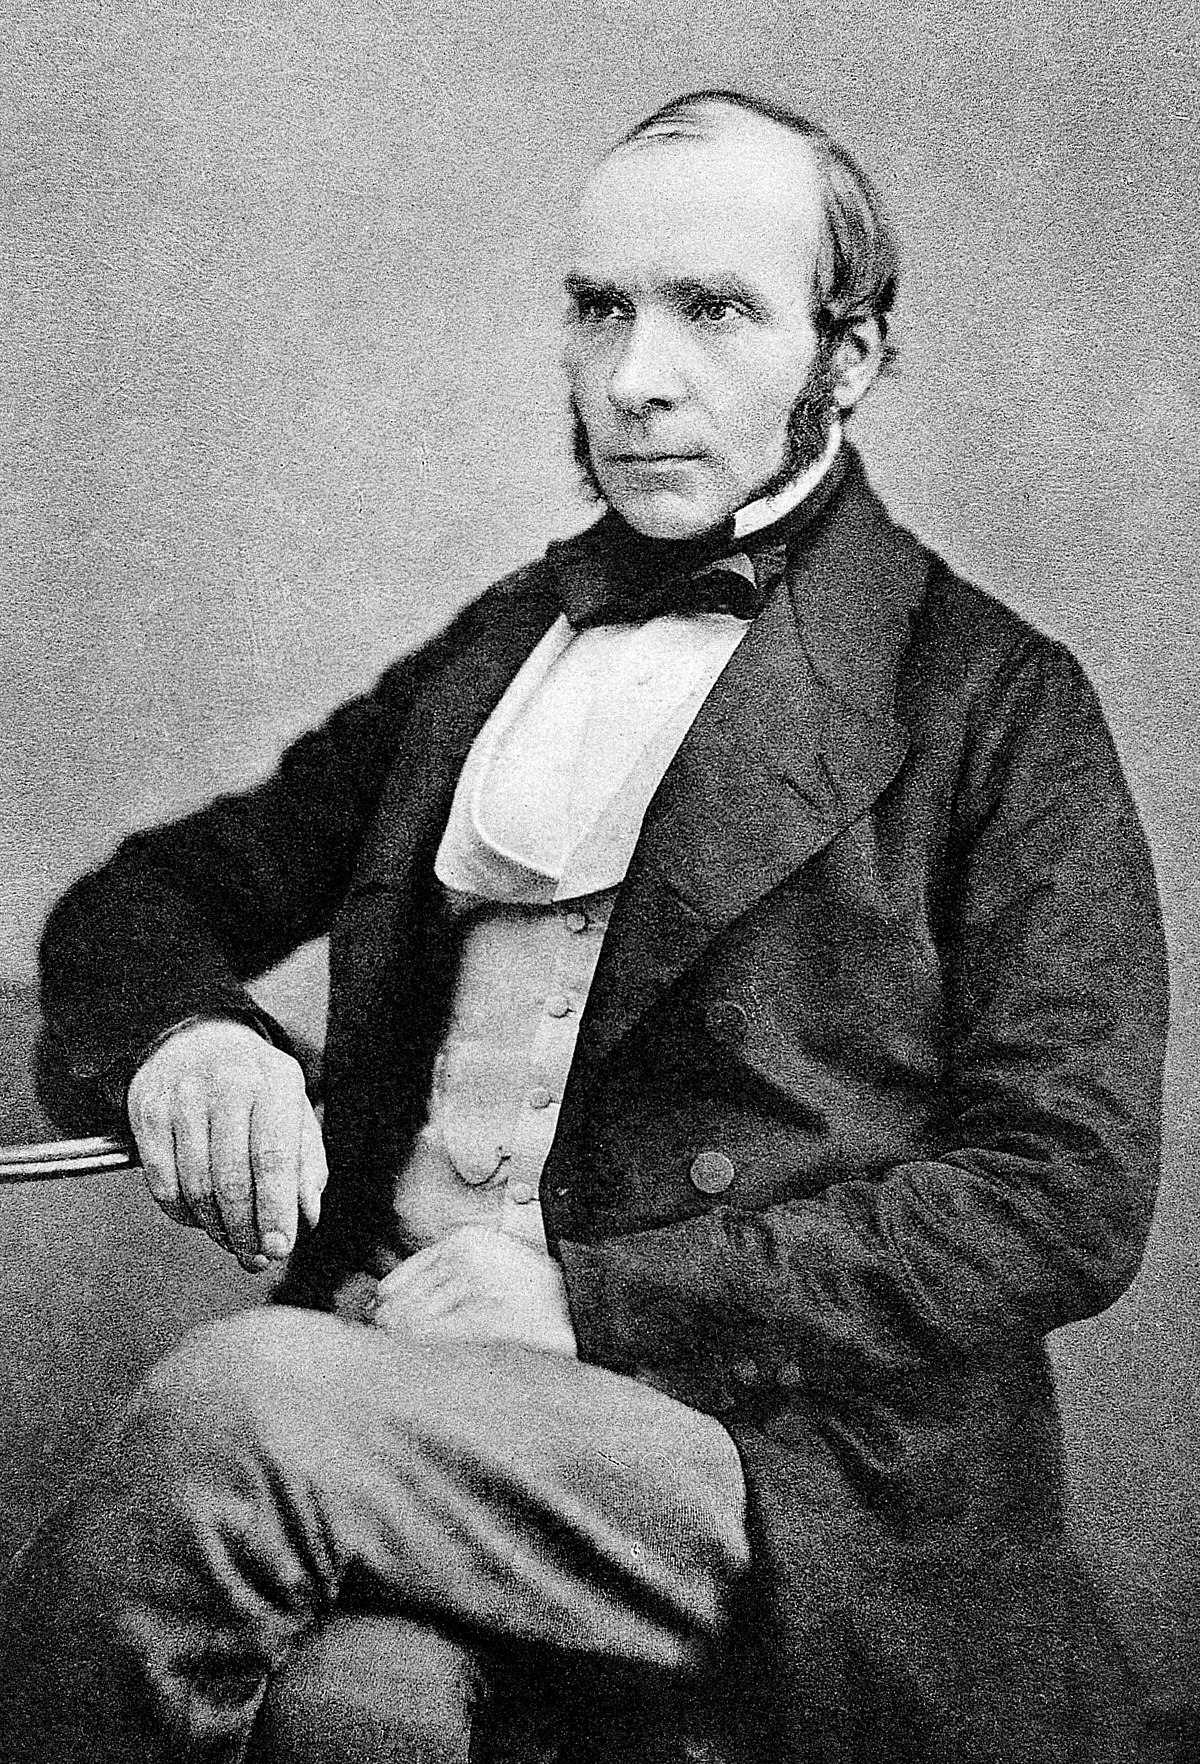
\includegraphics{./images/John_Snow.jpg}

}

\caption{John Snow}

}

\end{minipage}%
%
\begin{minipage}[b]{0.50\linewidth}

{\centering 

\raisebox{-\height}{

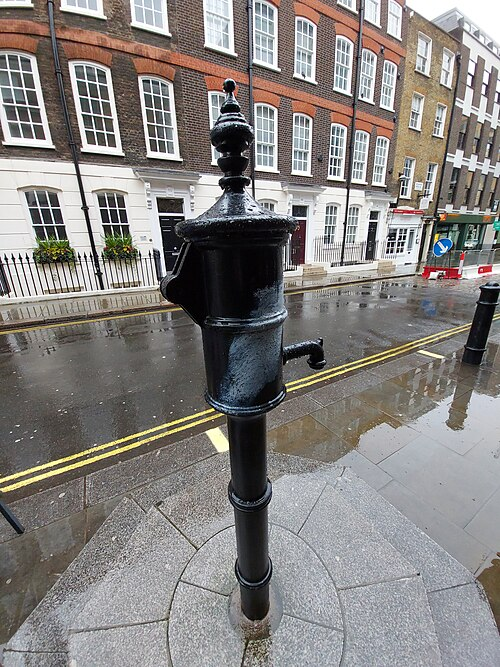
\includegraphics{./images/john_snow_pump.jpg}

}

\caption{His study pump}

}

\end{minipage}%

\end{figure}

\textbf{Jhon Snow} example: For short, in 19th century, cholera expand
all over Europe and UK. Estimated 15,000 recorded deaths in London in
1848-9. Snow (an anaesthetist) came up with some hypothesis:

\begin{itemize}
\item
  that cholera can be communicated from the sick to the healthy
\item
  that disease is communicated by ``morbid matter'' which has the
  property of multiplying in the body of the person it attacks
\item
  that the morbid matter producing cholera must be introduced into the
  alimentary canal
\item
  water supplies appeared to be able to disseminate the morbid matter
  from the sick to the healthy
\end{itemize}

In 1853, cholera reappeared and Snow started his study. First he did a
descriptive study by collecting information on cholera deaths, where
they live and the population of the area. Then he look at the
association of the water sources and the risk of death from cholera.

\textbf{Comparison} is fundamental to epidemiology Just as Snow did, by
looking at the difference of risk between the groups using different
water sources, we can find the risk factors of a disease. However, in
reality, comparison is also the most challenge of epidemiology with many
sources of confusion and error.

\textbf{The two key elements} In most epidemiological studies, we would
measure 2 key elements which are the exposure and the outcome.

\begin{itemize}
\item
  The exposure (sometimes called risk factor or determinant) is any
  factor that may influence the outcome.
\item
  The outcome is the disease, or event, or health-related state, that we
  are interested in.
\end{itemize}

\hypertarget{what-is-the-role-of-epidemiology}{%
\section{what is the role of
Epidemiology?}\label{what-is-the-role-of-epidemiology}}

Epidemiology has four major functions:

\begin{itemize}
\item
  to \textbf{describe} patterns of health and disease within populations
\item
  to \textbf{interpret} these differences
\item
  to \textbf{apply} our results to public health practice, and
\item
  to \textbf{evaluate} the effect of health-related interventions
\end{itemize}

\hypertarget{basic-epidemilogical-study-types}{%
\section{Basic Epidemilogical study
types}\label{basic-epidemilogical-study-types}}

\begin{figure}

{\centering \includegraphics{./images/study_types.gif}

}

\end{figure}

This epidemiological studies family tree is simpler than the one
introduced by Ronald.

\hypertarget{measures-of-occurrence}{%
\chapter{Measures of Occurrence}\label{measures-of-occurrence}}

In Epidemiology, \textbf{population} is a group of people who share
characteristics or meet criteria that define membership in the
population (Lash et al. 2021).

Three common terms:

\begin{itemize}
\item
  The \emph{source population} is the population from which persons will
  be sampled and included in a measurement of disease frequency
\item
  The \emph{study population} (population at risk) is the subset, up to
  a complete census, of the source population whose experience is
  included in a measurement of disease frequency
\item
  The \emph{target population} comprises the persons for whom
  information gleaned by the measurement of disease frequency will be
  relevant
\end{itemize}

\textbf{Case} (or the outcome) definition should contain:

\begin{itemize}
\item
  The method(s) used to identify a case. The procedures or instruments
  that have been used to identify a case.
\item
  The boundaries of a case. The cut-off point to be a case or non-case.
\item
  The unit of analysis(person, a household\ldots{} )
\end{itemize}

Note: How we define a case influences how we define the study
population.

\hypertarget{prevalence}{%
\section{Prevalence}\label{prevalence}}

The total number of individuals who have the condition (e.g., disease,
exposure, attribute) at a particular time (or during a particular
period) divided by the population at risk of having the condition at
that time or midway through the period. (Porta 2014)

\textbf{Point prevalence} (often used) is the proportion of persons in a
defined population that has the outcome under study at a specific point
in time

\[\text{Point prevalence} =  \frac{\text{Number of cases at time t}}{\text{Study population at time t}}\]

\begin{tcolorbox}[enhanced jigsaw, bottomtitle=1mm, breakable, colframe=quarto-callout-important-color-frame, leftrule=.75mm, opacityback=0, opacitybacktitle=0.6, left=2mm, colbacktitle=quarto-callout-important-color!10!white, coltitle=black, rightrule=.15mm, toptitle=1mm, colback=white, titlerule=0mm, title=\textcolor{quarto-callout-important-color}{\faExclamation}\hspace{0.5em}{Important}, arc=.35mm, bottomrule=.15mm, toprule=.15mm]

In the denominator, the study population at time t means excluding
individuals lost to follow up and death.

\end{tcolorbox}

Example:

\textbf{Period prevalence} is the number of cases in a population over a
defined period of time. Not often used.

\hypertarget{incidence}{%
\section{Incidence}\label{incidence}}

\textbf{Incidence risk} is the proportion of new cases that occur in a
population initially free of the condition during a specified period of
time.

\[\text{Incidence risk}  = \frac{\text{number of new cases in a defined time period}}{\text{population at risk at the beginning of the period}}\]

\begin{tcolorbox}[enhanced jigsaw, bottomtitle=1mm, breakable, colframe=quarto-callout-important-color-frame, leftrule=.75mm, opacityback=0, opacitybacktitle=0.6, left=2mm, colbacktitle=quarto-callout-important-color!10!white, coltitle=black, rightrule=.15mm, toptitle=1mm, colback=white, titlerule=0mm, title=\textcolor{quarto-callout-important-color}{\faExclamation}\hspace{0.5em}{Important}, arc=.35mm, bottomrule=.15mm, toprule=.15mm]

The incidence risk is a measure of \textbf{NEW} cases, and point
prevalence a measure of \textbf{EXISTING} cases.

\end{tcolorbox}

\textbf{Mortality rate} (or death rate) is a measure of the incidence
risk of dying during a defined period of time.

\textbf{Attack rate} is a special kind of incidence risk. It is used in
the context of outbreaks or epidemics of infectious diseases. It is the
number of new cases occurring in the duration of the outbreak divided by
the population at risk in the start of the outbreak.

\textbf{Case fatality rate} the proportion of cases of a specified
condition that are fatal within a specified time.

\[\text{Case fatality rate} = \frac{\text{Number of deaths from a disease(in a given period)}}{\text{Number of diagnosed cases of that disease (in the same period)}}\]

\begin{tcolorbox}[enhanced jigsaw, bottomtitle=1mm, breakable, colframe=quarto-callout-important-color-frame, leftrule=.75mm, opacityback=0, opacitybacktitle=0.6, left=2mm, colbacktitle=quarto-callout-important-color!10!white, coltitle=black, rightrule=.15mm, toptitle=1mm, colback=white, titlerule=0mm, title=\textcolor{quarto-callout-important-color}{\faExclamation}\hspace{0.5em}{Important}, arc=.35mm, bottomrule=.15mm, toprule=.15mm]

Even though these measures are called rates but actually they are risk.
The denominator does not include time (e.g person-year)

\[\text{Mortality rate} = \text{(Incidence risk ) x (Case fatality rate)}\]

\end{tcolorbox}

\textbf{Incidence rate} relates the number of new cases to the total
person-time at risk.

\[\text{Incidence rate} = \frac{\text{Number of new cases in a defined time period}}{\text{Total person-time at risk}}\]

\textbf{Example 1:}

\begin{figure}

{\centering 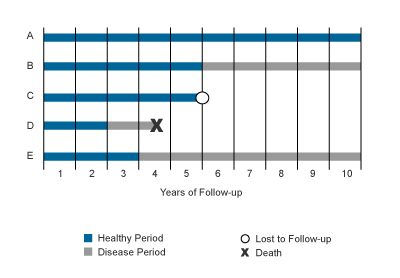
\includegraphics{./images/incidence_risk.png}

}

\end{figure}

\[\text{Prevalence at year 7} = \frac{1}{3}\]
\[\text{Incidence risk over 10 years perios} = \frac{3}{5}\]

\[\text{Incidence rate over 10 years period} = \frac{3}{25}\text{per person-year}\]
\textbf{Example 2}: Incidence rate

\begin{figure}

{\centering 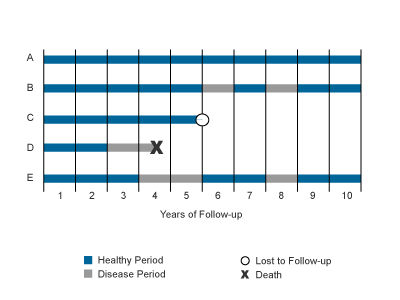
\includegraphics{./images/incidence_rate.png}

}

\end{figure}

\[\text{Incidence rate over 10 years period} = \frac{5}{32} \text{per person-year}\]

\hypertarget{odds}{%
\section{Odds}\label{odds}}

Odds is the ratio of the probability of occurrence of an event to that
of nonoccurrence. (Porta 2014)

\[\text{Odds} = \frac{\text{number of cases}}{\text{number of non-cases}}\]

\begin{tcolorbox}[enhanced jigsaw, bottomtitle=1mm, breakable, colframe=quarto-callout-important-color-frame, leftrule=.75mm, opacityback=0, opacitybacktitle=0.6, left=2mm, colbacktitle=quarto-callout-important-color!10!white, coltitle=black, rightrule=.15mm, toptitle=1mm, colback=white, titlerule=0mm, title=\textcolor{quarto-callout-important-color}{\faExclamation}\hspace{0.5em}{Important}, arc=.35mm, bottomrule=.15mm, toprule=.15mm]

The odds of becoming a case is rarely used as a measure of occurrence on
its own. However, it is an important component of a measure of effect,
the odds ratio

\end{tcolorbox}

\hypertarget{comparison}{%
\section{Comparison}\label{comparison}}

The prevalence (P) quantifies all the people with an outcome at a point
in time. It is influenced by the occurrence of new cases (incidence, I)
and the duration of each case (D): \textbf{P= I x D}.

As so many factors influence prevalence, it is difficult to interpret
comparative studies of the prevalence of the same condition in different
settings.

It can also be difficult to interpret the reasons for a change in the
prevalence of a condition in the same location.

However, prevalence studies provide useful information about the state
of health of a community at a particular point in time, and so are
useful for evaluating health-care needs and planning health service
provision.

This is particularly important for chronic conditions that require
health care resources throughout their duration.

The prevalence can also be used to evaluate the impact of preventative
measures aimed at reducing the burden of a disease or condition in a
community.

However, because of the number of factors that influence prevalence, any
comparative results need to be interpreted with caution.

\begin{tcolorbox}[enhanced jigsaw, bottomtitle=1mm, breakable, colframe=quarto-callout-important-color-frame, leftrule=.75mm, opacityback=0, opacitybacktitle=0.6, left=2mm, colbacktitle=quarto-callout-important-color!10!white, coltitle=black, rightrule=.15mm, toptitle=1mm, colback=white, titlerule=0mm, title=\textcolor{quarto-callout-important-color}{\faExclamation}\hspace{0.5em}{Important}, arc=.35mm, bottomrule=.15mm, toprule=.15mm]

\textbf{Prevalence} is useful for chronic diseases that require health
resource. It can be used for evaluating health-care needs and planning.

\textbf{Incidence risk} provides good evidence for studying causality
when the outcome of interest is uncommon or acute diseases and the
population is static.

\textbf{Incidence rate} is useful when the population is dynamic, the
outcome of interest is common or the population at high risk(the number
of new cases will be relatively high) or can occur many times.

\end{tcolorbox}

\hypertarget{measures-of-effectassociation}{%
\chapter{Measures of
Effect/Association}\label{measures-of-effectassociation}}

As mentioned in \protect\hyperlink{fundamental-epidemiology}{Fundamental
Epidemiology} section, comparison is fundamental in epidemiological
studies. When interpreting the results from both observational and
analytical studies, we typically use some sort of comparison.

In analytical studies, we often aim investigate risk factors of an
outcome. If we suspect that a particular factor may be causing a
specific outcome, we first look for an association between the factor
and the outcome. To do this, we compare the occurrence of the outcome in
a group of people that has been `exposed' to the factor, with the
occurrence in a group of people that has not been `exposed'. We use
ratio measures or difference measures.

\textbf{Ratio}: The value obtained by dividing one quantity by another
(Porta 2014). We can use the ratio to compare any type of measure
occurrence: Prevalence, Incidence or Odds between 2 populations.

\textbf{Prevalence ratio}

The prevalence ratio is sometimes used in health-service planning to
compare the burden of a condition in different groups. Prevalence is
less useful than incidence in trying to establish the effect of an
exposure, because prevalence depends on both incidence and duration

\[\text{Prevalence ratio} = \frac{\text{prevalence in population or group A}}{\text{prevalence in population or group B}}\]

\textbf{Risk ratio}

\[\text{RR} = \frac{\text{incidence risk in exposed population}}{\text{incidence risk in unexposed population}}\]

\textbf{Rate ratio}

\[\text{RR} = \frac{\text{incidence rate in exposed population}}{\text{incidence rate in unexposed population}}\]

\textbf{Odds ratio}

\[\text{OR} = \frac{\text{odds of outcome in exposed individuals}}{\text{odds of outcome in unexposed individuals}}\]

\textbf{Odds ratio in Case-Control Study}

\[\text{OR} = \frac{\text{odds of exposure in cases (people with the outcome)}}{\text{odds of exposure in controls (people without the outcome)}}\]

\begin{tcolorbox}[enhanced jigsaw, bottomtitle=1mm, breakable, colframe=quarto-callout-important-color-frame, leftrule=.75mm, opacityback=0, opacitybacktitle=0.6, left=2mm, colbacktitle=quarto-callout-important-color!10!white, coltitle=black, rightrule=.15mm, toptitle=1mm, colback=white, titlerule=0mm, title=\textcolor{quarto-callout-important-color}{\faExclamation}\hspace{0.5em}{Important}, arc=.35mm, bottomrule=.15mm, toprule=.15mm]

For rare outcomes in static populations (case-control studies), Odds
ratio is almost similar to Risk ratio and rate ratio. Some people just
call them all \textbf{Relative risk}.

\end{tcolorbox}

\hypertarget{interpretation-of-ratio-measures-association}{%
\section{Interpretation of Ratio Measures
(Association)}\label{interpretation-of-ratio-measures-association}}

To estimate an association, we need to answer 2 questions:

\textbf{Is there an association?}

\begin{itemize}
\item
  Relative Risk = 1 : No association
\item
  Relative Risk \textgreater{} 1 : The risk/rate/odds of the outcome in
  the exposed group is greater than that in the unexposed group
\item
  Relative Risk \textless{} 1 : The risk/rate/odds of the outcome in the
  exposed group is less than that in the unexposed group. The exposure
  is a \textbf{protective factor} for the outcome.
\end{itemize}

\textbf{Example}

\textbf{AND}

\textbf{How does this association mean?}

To conclude the association between exposure and outcome, we need to
consider other aspects: random error, bias, confounding. Bias and
confounding will be discussed in more details in the following sections.
Random error is related to estimates obtained by chance. We use
Confidence Intervals to assess the level of certainty.

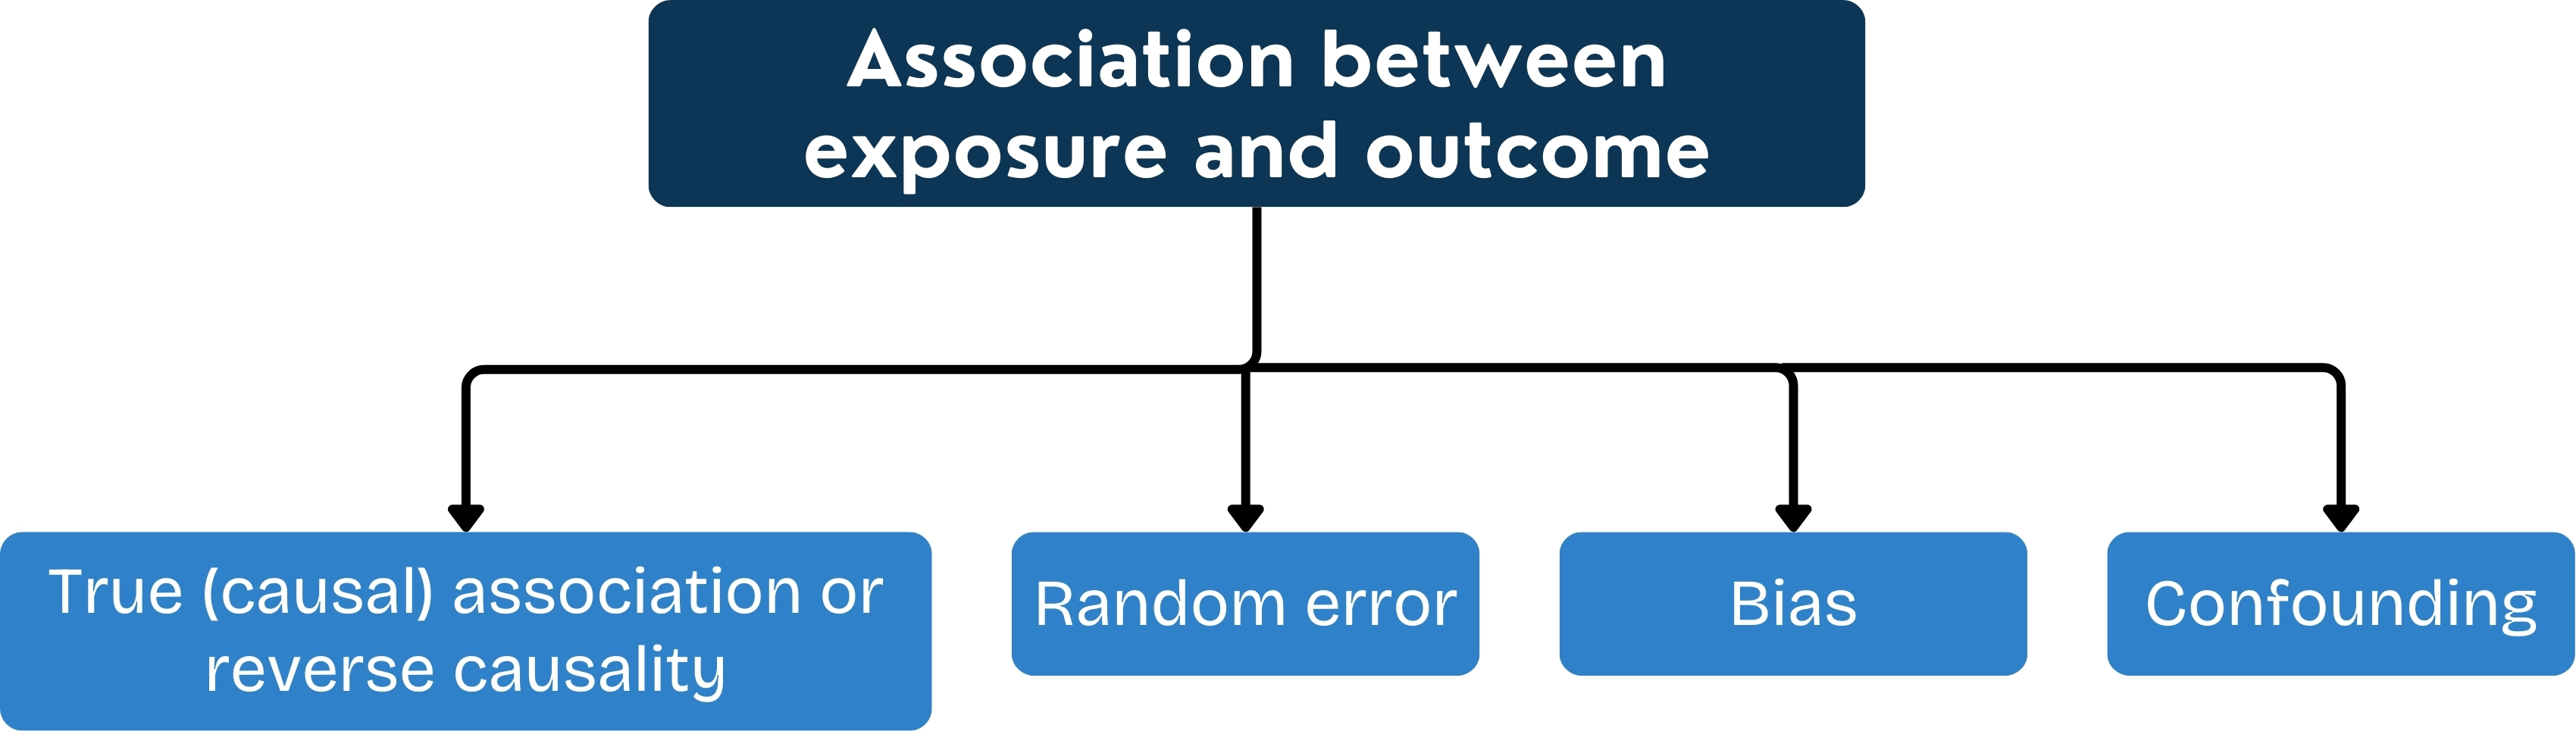
\includegraphics{./images/association.jpg}

\hypertarget{difference-measures}{%
\section{Difference measures}\label{difference-measures}}

\[\text{Absolute difference} = \text{occurrence (exposed) − occurrence (unexposed)}\]

\[\text{Risk/Rate difference} = \text{Risk/Rate (exposed) − Risk/Rate (unexposed)}\]

\textbf{Interpretation}

The difference measures are useful when we already have information that
suggests that there is a \textbf{causal relationship} between the
exposure and the outcome. The difference measures sometimes is called
\textbf{attributable risk} or rate.

\begin{itemize}
\item
  If the difference is \textbf{positive}, this estimates \textbf{the
  excess occurrence} of the outcome in the exposed group. When the
  causality is true, this equivalent to the number of cases in the
  exposed group that are \textbf{caused} by the exposure.
\item
  If the difference is \textbf{negative}, this estimates \textbf{the
  reduction occurrence} of the outcome in the exposed group. When the
  causality is true, this equivalent to the number of cases in the
  exposed group that have been \textbf{prevented} by the exposure.
\end{itemize}

\begin{tcolorbox}[enhanced jigsaw, bottomtitle=1mm, breakable, colframe=quarto-callout-important-color-frame, leftrule=.75mm, opacityback=0, opacitybacktitle=0.6, left=2mm, colbacktitle=quarto-callout-important-color!10!white, coltitle=black, rightrule=.15mm, toptitle=1mm, colback=white, titlerule=0mm, title=\textcolor{quarto-callout-important-color}{\faExclamation}\hspace{0.5em}{Important}, arc=.35mm, bottomrule=.15mm, toprule=.15mm]

The difference measure does not give any information about the impact of
the exposure on the number of cases in the population as a whole. This
depends on the prevalence of the exposure in the population.

There are more concepts about attributable but I do not present in this
material: Attributable fraction in the exposed group, preventable
fraction, population attributable risk, population attributable
fraction.

\end{tcolorbox}

\hypertarget{comparison-between-ratio-and-difference-measures}{%
\section{Comparison between Ratio and Difference
measures}\label{comparison-between-ratio-and-difference-measures}}

Ratio measures and difference measures are influenced by different
factors and provide different types of information.

\textbf{Ratio measures} estimate the strength of association between an
exposure and an outcome. We use a ratio measure in analytical studies as
one piece of evidence in judging whether an exposure causes an outcome.

\textbf{Difference measures} quantify the difference in incidence
between an exposed and an unexposed population. We use difference
measures when \emph{a causal association between an exposure and an
outcome has already been established}, to estimate the risk that is
attributable to exposure in the exposed group.

The measures covered in this session are appropriate where the exposure
measure is \textbf{a categorical variable}. They cannot, therefore, be
used to analyse continuous exposure variables

\begin{tcolorbox}[enhanced jigsaw, bottomtitle=1mm, breakable, colframe=quarto-callout-important-color-frame, leftrule=.75mm, opacityback=0, opacitybacktitle=0.6, left=2mm, colbacktitle=quarto-callout-important-color!10!white, coltitle=black, rightrule=.15mm, toptitle=1mm, colback=white, titlerule=0mm, title=\textcolor{quarto-callout-important-color}{\faExclamation}\hspace{0.5em}{Important}, arc=.35mm, bottomrule=.15mm, toprule=.15mm]

\textbf{Terminology}

There are three commonly used measures of \textbf{disease frequency} in
epidemiology: we have called these the odds, the risk, and the rate. The
numerator in all of three of these is the number of cases occurring
within a defined period of time. The difference is in the denominator:
the odds uses the number of non-cases within the same time period, the
risk uses the number of individuals at the beginning of the follow-up
period, and the rate uses the person-time at risk during the follow-up
period. The ratio of odds, risks or rates between two groups gives the
respective \textbf{measures of effect}: the odds ratio, the risk ratio
and the rate ratio.

In the literature, however, it is common to see these terms used
interchangeably, which can cause confusion. In particular, the term
\textbf{risk} is often used generically to refer to any of the above
measures of \textbf{disease frequency}. To complicate things further,
some of these measures have other names: the risk is also sometimes
referred to as the cumulative risk, while the rate is sometimes known as
the incidence density. In infectious disease epidemiology, the force of
infection is used to describe the rate at which susceptible individuals
become infected.

\textbf{Make it clear what you are measuring in your study}

\end{tcolorbox}

\hypertarget{bias}{%
\chapter{Bias}\label{bias}}

There are more than 20 types of bias in the Dictionary of Epidemiology
book (Porta 2014). They are defined inconsistently in different fields.
Some authors regard confounding as a type of bias.

In Epidemiology, bias refers to any systematic error in the design or
conduct of an epidemiological study that results in an incorrect
estimate of the association between exposure and outcome (risk of
disease).

In confounding, the associations do exist in the population of interest,
however, they are not causal but rather explained by association with
another factor. The effect of confounding can be controlled in our
analysis.

By contrast, when bias occurs the associations are not `there' at all,
they only exist within your study. A biased study is one that does not
give a true representation of the situation we want to describe or the
association we want to analyse. We cannot control for the effect of bias
in our analysis. Instead, we need to identify potential sources of bias
and try to minimise them.

In this section, I will summary 2 main types of bias: Selection bias and
Information bias.

\hypertarget{selection-bias}{%
\subsection{Selection Bias}\label{selection-bias}}

Selection bias refers to error due to systematic differences in
characteristics between those who take part in a study and those who do
not, such that

\begin{itemize}
\tightlist
\item
  the people who are selected to participate in a study are not
  representative of the reference population
\end{itemize}

or, in analytic studies,

\begin{itemize}
\tightlist
\item
  the comparison groups are not comparable
\end{itemize}

\textbf{Descriptive studies} (cross-sectional or cohort studies): bias
occurs if the study population is not representative of the source
population (the population that we draw our study population from). In
cross-sectional studies, selection bias may occur because rarely 100\%
of individuals participate, and if there are differences in
characteristics between those who participate and those who do not.

Example:

\textbf{Analytical Studies}:

\textbf{1. Case control studies}

\begin{itemize}
\item
  cases are not representative of all cases within a defined population
  (all eligible cases), or
\item
  controls are not representative of the population which produced the
  cases.
\end{itemize}

\textbf{2. Cohort Studies}

\begin{itemize}
\item
  poor choice of the unexposed group, or
\item
  differences in follow-up between the comparison groups
\end{itemize}

\textbf{Missing data} can be considered as a form of selection bias. It
is important to describe the extent and the patterns of missing data,
comparing individuals with and without missing data for key variables.
This helps us to make assumptions about the nature of the missing data,
and to assess the effect the missingness could have on our analyses.

\hypertarget{information-bias}{%
\subsection{Information Bias}\label{information-bias}}

\textbf{Reporting bias}

\begin{itemize}
\item
  when study participants with a specific health outcome report previous
  exposures with a different degree of accuracy to those without the
  outcome, or
\item
  when study participants who have experienced a specific exposure
  report subsequent health events with a different degree of accuracy to
  those who have not experienced the exposure.
\end{itemize}

\textbf{Observer bias}

\begin{itemize}
\item
  in case-control or cross-sectional studies, when the accuracy of
  exposure data recorded by the investigator differs systematically
  between study participants in different outcome groups or
\item
  in cohort or intervention studies, when the accuracy of outcome data
  recorded by the investigator differs systematically between
  individuals in different exposure groups
\end{itemize}

\hypertarget{stratergies-to-minimise-bias}{%
\section{Stratergies to minimise
Bias}\label{stratergies-to-minimise-bias}}

\hypertarget{avoiding-selection-bias}{%
\subsection{Avoiding selection bias}\label{avoiding-selection-bias}}

\begin{itemize}
\item
  in descriptive studies, that study participants are representative of
  the target population and the response rates are as high as possible.
\item
  in case-control studies, that the controls represent the population
  which produced the cases.
\item
  in cohort studies, loss to follow-up is minimised.
\end{itemize}

\hypertarget{avoiding-information-bias}{%
\subsection{Avoiding information bias}\label{avoiding-information-bias}}

\begin{itemize}
\item
  blinding of study participants (where feasible) helps to avoid recall
  bias
\item
  blinding of observers helps to prevent classification of exposure or
  outcome being influenced by knowledge of the other
\item
  using objective records to document exposure rather than relying on
  recall
\item
  collecting data on exposure as near as possible to the time of
  exposure (when recall is likely to be more accurate)
\item
  standardising questionnaires and training interviewers, so that all
  study participants are asked the same questions in the same way
\item
  good questionnaire design, for example using closed questions
  (i.e.~questions with a limited range of possible answers)
\item
  using automated measuring devices to reduce observer bias
\end{itemize}

\hypertarget{confounders-and-effect-modification}{%
\chapter{Confounders and Effect
Modification}\label{confounders-and-effect-modification}}

\hypertarget{measurement-errors}{%
\chapter{Measurement Errors}\label{measurement-errors}}

\hypertarget{study-design}{%
\chapter{Study design}\label{study-design}}

\includegraphics{./images/study_types.gif}

\part{Study designs}

\hypertarget{cross-sectional-study}{%
\chapter{Cross-sectional study}\label{cross-sectional-study}}

\textbf{Design}

In a cross-sectional study, we measure the frequency of a particular
exposure(s) and / or outcome(s) in a defined population at a particular
point in time. Sometimes it is called prevalence study.

In a descriptive cross-sectional study, we simply describe the frequency
of the exposure(s) or outcome(s) in a defined population.

In an analytic cross-sectional study, we simultaneously collect
information on both the outcome of interest potential risk factor(s) in
a defined population. We then compare the prevalence of the outcome in
the people exposed to each risk factor with the prevalence in those not
exposed.

\textbf{Why do Cross-sectional study?}

\textbf{Descriptive study}

\begin{itemize}
\item
  as the study measures the prevalence, it is useful for health planners
  who need to know the burden of specific conditions in order to plan
  preventive and curative services.
\item
  some cross-sectional studies also collect data on the utilisation of
  preventive and curative services. it's useful for predicting health
  care needs and establishing health-care priorities.
\item
  Some studies collect information about the knowledge, attitudes and
  practices of a population in relation to a particular health-related
  outcome. it's useful for the development of population-level health
  education campaigns.
\end{itemize}

\begin{tcolorbox}[enhanced jigsaw, bottomtitle=1mm, breakable, colframe=quarto-callout-important-color-frame, leftrule=.75mm, opacityback=0, opacitybacktitle=0.6, left=2mm, colbacktitle=quarto-callout-important-color!10!white, coltitle=black, rightrule=.15mm, toptitle=1mm, colback=white, titlerule=0mm, title=\textcolor{quarto-callout-important-color}{\faExclamation}\hspace{0.5em}{Important}, arc=.35mm, bottomrule=.15mm, toprule=.15mm]

Cross-sectional studies are not suitable for describing the frequency of
rare exposures or outcomes.

\end{tcolorbox}

\textbf{Analytical study}

\begin{itemize}
\item
  as the study measures the prevalence at a particular time point, it
  does not provide strong evidence about the causality. It can be
  difficult to establish the time sequence of events: the exposure may
  be a consequence rather than a cause of the outcome (\textbf{reverse
  causality})
\item
  We cannot use cross-sectional study to test a hypothesis. Instead, we
  use it to generate hypothesis.
\end{itemize}

\hypertarget{main-steps-in-conducting-a-cross-sectional-study}{%
\section{Main steps in conducting a Cross-sectional
study}\label{main-steps-in-conducting-a-cross-sectional-study}}

\textbf{Step 1: Defining the study question}

\textbf{Step 2: Defining the target population selecting the study
population}

Refer to \protect\hyperlink{measures-of-occurrence}{Measures of
Occurrence} section for definition of different concepts of population.
Basically, the target population is the group to which we can generalise
our study results, while the study population consists of the
individuals we intend to include in our study. If the target population
is small, we can study the entire population. However, in practice, the
study population is usually a sample of the target population.

It is important to select the sample as representative of the target
population, otherwise we will introduce selection bias in our study. The
best way to ensure this is random sampling: Simple random sampling,
Systematic sampling, Stratified sampling, Multi-stage sampling.

Most of the time, not all individuals of our target population will
participate in our study even though we have tried our best. We should
collect as much as possible information about those who do not
participate. If there is systematic different characteristics between
those who participate and those who do not, there is selection bias in
our study.

\textbf{Step 3: Collecting data}

\textbf{Step 4: Analysing data}

\textbf{Step 5: Interpreting results}

\hypertarget{strength-and-weakness}{%
\section{Strength and Weakness}\label{strength-and-weakness}}

\hypertarget{cohort-study}{%
\chapter{Cohort study}\label{cohort-study}}

\hypertarget{case-control-study}{%
\chapter{Case-control study}\label{case-control-study}}

\hypertarget{intervention-study}{%
\chapter{Intervention study}\label{intervention-study}}

\bookmarksetup{startatroot}

\hypertarget{summary}{%
\chapter*{Summary}\label{summary}}
\addcontentsline{toc}{chapter}{Summary}

\markboth{Summary}{Summary}

In summary, this book has no content whatsoever.

\begin{Shaded}
\begin{Highlighting}[]
\DecValTok{1} \SpecialCharTok{+} \DecValTok{1}
\end{Highlighting}
\end{Shaded}

\begin{verbatim}
[1] 2
\end{verbatim}

\bookmarksetup{startatroot}

\hypertarget{references}{%
\chapter*{References}\label{references}}
\addcontentsline{toc}{chapter}{References}

\markboth{References}{References}

\hypertarget{refs}{}
\begin{CSLReferences}{1}{0}
\leavevmode\vadjust pre{\hypertarget{ref-lash_modern_2021}{}}%
Lash, Timothy L., Tyler J. VanderWeele, Sebastien Haneuse, and Kenneth
J. Rothman. 2021. \emph{Modern Epidemiology.} Fourth edition / Timothy
L. Lash, Tyler J. VanderWeele, Sebastien Haneuse, Kenneth J. Rothman.
Philadelphia: Wolters Kluwer.

\leavevmode\vadjust pre{\hypertarget{ref-porta_dictionary_2014}{}}%
Porta, Miquel. 2014. \emph{A Dictionary of Epidemiology.} Oxford
University Press.

\end{CSLReferences}



\end{document}
